\subsection{Conditional image generation with CLIP Using Diffusion Models}
\begin{frame}[allowframebreaks]{Conditional image generation with CLIP Using Diffusion Models}
    \textbf{Conditional image generation with CLIP Using Diffusion Models} combines the power of diffusion models for image synthesis with CLIP's ability to understand and condition on text prompts, enabling the generation of images that align with specific textual descriptions.

    \begin{itemize}
        \item \textbf{Diffusion Models:} These models generate images by iteratively refining noise into coherent images, allowing for high-quality synthesis.
        \item \textbf{CLIP:} Provides text embeddings that guide the diffusion process, ensuring that the generated images match the desired attributes described in the text.
        \item \textbf{Applications:} Image synthesis, style transfer, and content-aware editing based on textual prompts.
    \end{itemize}
\framebreak
    \begin{figure}
        \centering
        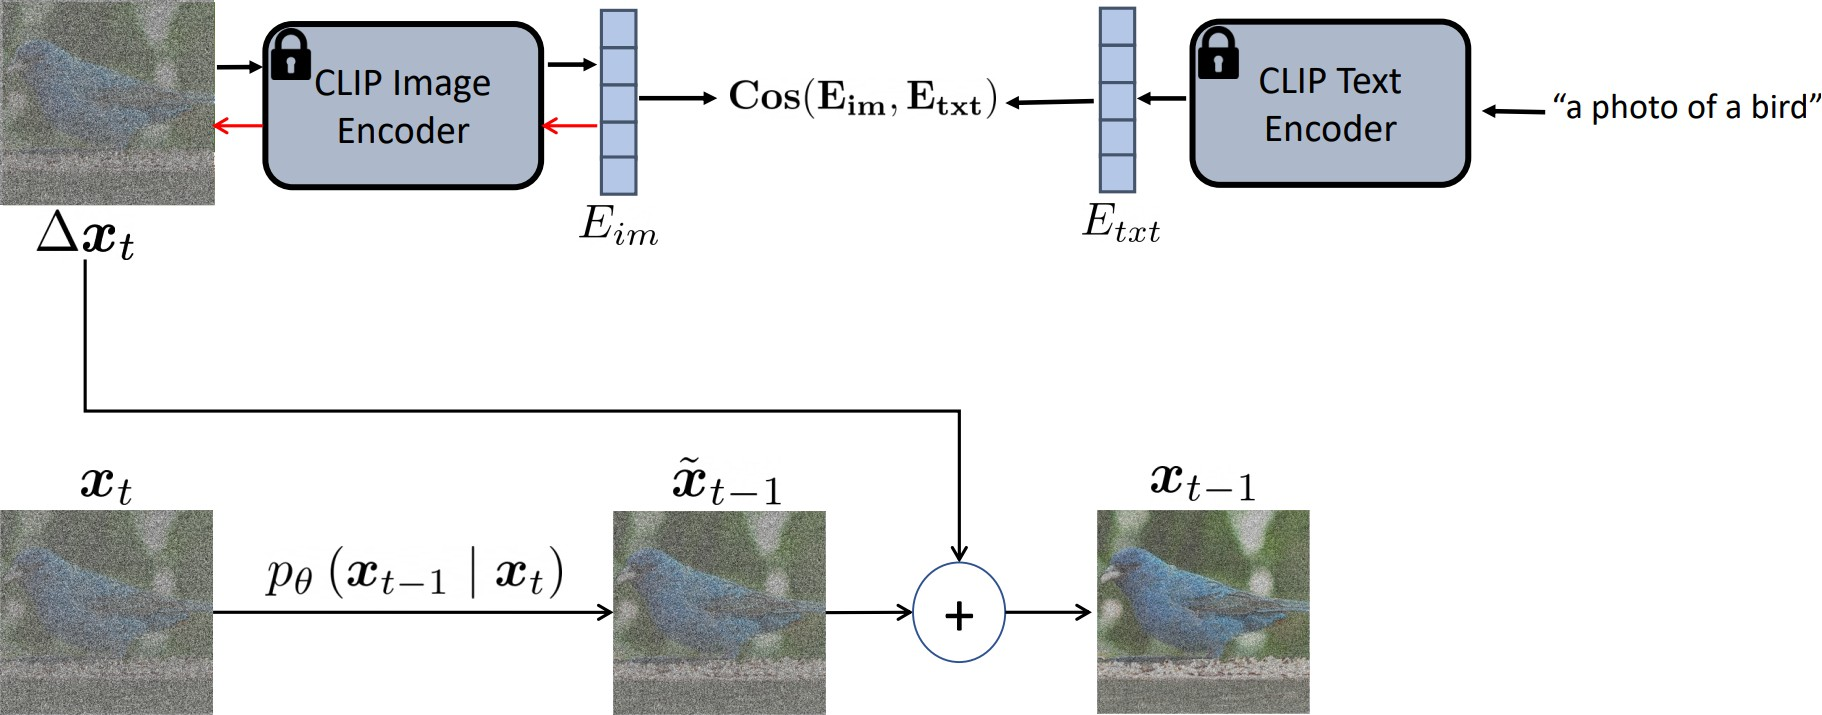
\includegraphics[width=1\textwidth,height=0.8\textheight,keepaspectratio]{images/video/slide_69_1_img.jpg}
    \end{figure}
    {\footnotesize{[Diffusion Models Beat GANs on Image Synthesis, Dhariwal and Nichol et al. NeurIPS 2021]}}
\framebreak
    \begin{figure}
        \centering
        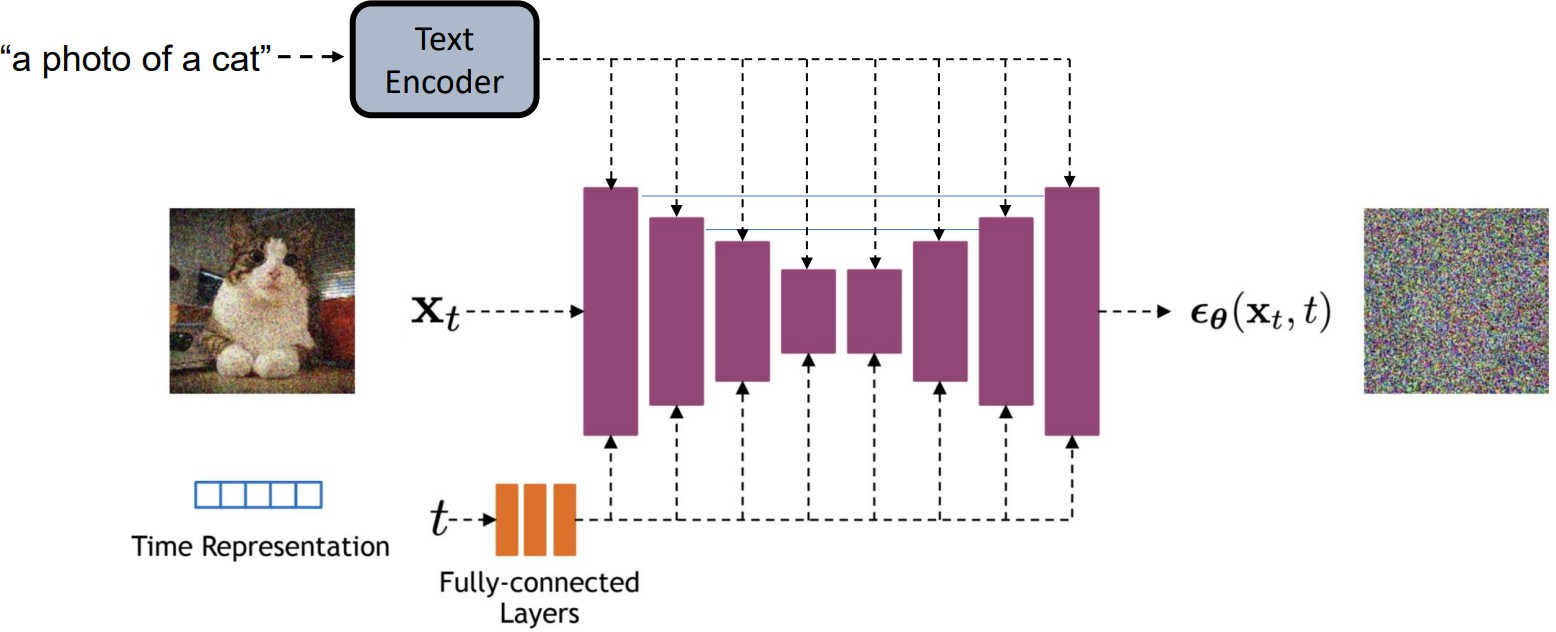
\includegraphics[width=1\textwidth,height=0.9\textheight,keepaspectratio]{images/video/slide_70_1_img.jpg}
    \end{figure}
\end{frame}